\subsection{Ablation of the source and endpoint corrections}\label{sec:source-head-ablation}
We compare four settings: Gaussian or harmonic source, each with or without
the geometric and physical correction block. These experiments use one-pass
EGNN flow models. Within each fit, both sources receive the same frozen
correction weights, learned with the self-conditioned FM. This separates the
source choice from correction fitting.

\begin{figure}[!htbp]\centering
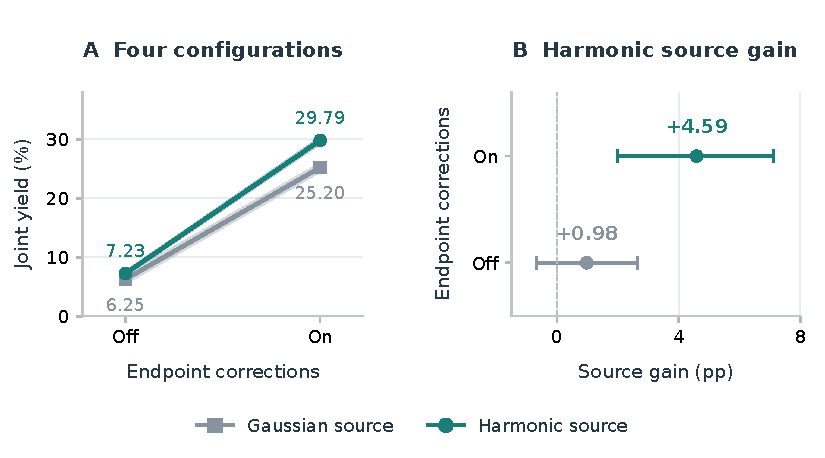
\includegraphics[width=\linewidth]{../research/figures/geometric_followups_v1/components.pdf}
\caption{Contributions of the source and endpoint corrections. (A) Mean joint
graph-and-force yield for four settings; faint lines retain both fits.
(B) Harmonic-minus-Gaussian gains, with nominal 95\% intervals from resampling
fits and compositions. Each setting uses 2,048 outputs on the same 64 compositions.}
\label{fig:source-head-ablation}\end{figure}

The correction block raises joint yield from 6.25 to 25.20\% for Gaussian FM
and from 7.23 to 29.79\% for harmonic FM. With corrections active, the harmonic
source adds 4.59 points, with crossed 95\% interval $[2.00,7.13]$.
The source-only gain is 0.98 points, with interval $[-0.68,2.64]$.
Geometry-and-force yield changes from 1.51 to 6.40\% for Gaussian FM and
from 2.10 to 8.11\% for harmonic FM. Its smaller source gain with corrections,
1.71 points, has interval $[-1.46,4.69]$. The source benefit is clearest for
joint graph-and-force yield. Appendix~\ref{app:main-implementation} gives each fit;
Appendix~\ref{app:geometric-recovery} separates geometric and physical feedback.
